\section{Problem Formulation}
\label{sec:problem}
\subsection{From Outage to Average AoII}
Specializing the binary-source framework of~\cite{maatouk2020aoii,chen2021imperfect} to our slot-end update convention, write $q=q_\epsilon(\mathbf x)$. Since transmission outcomes are independent of the task source and past slots,~\eqref{eq:estimate}--\eqref{eq:aoii} imply
\begin{align}
 \Pr(A_t=1\mid A_{t-1}=0)&=\alpha q\triangleq\mu_0,\nonumber\\
 \Pr(A_t=a+1\mid A_{t-1}=a)&=(1-\alpha)q\triangleq\mu_1,
 \quad a\ge1.
 \label{eq:age-transitions}
\end{align}
All other transitions return to zero. The stationary probabilities are $\xi_0=(1-\mu_1)/(1-\mu_1+\mu_0)$ and $\xi_a=\xi_0\mu_0\mu_1^{a-1}$ for $a\ge1$. Therefore,
\begin{align}
 \overline\Delta_\epsilon^{\rm II}(\mathbf x)
 &\triangleq\lim_{N\to\infty}\frac1N
       \mathbb E\!\left[\sum_{t=1}^{N}TA_t\mid\mathbf x\right]\nonumber\\
 &=T\frac{\alpha q_\epsilon(\mathbf x)}
 {\left[1-(1-\alpha)q_\epsilon(\mathbf x)\right]
  \left[1-(1-2\alpha)q_\epsilon(\mathbf x)\right]}.
 \label{eq:mean-aoii}
\end{align}
For $0<\alpha\le1/2$,~\eqref{eq:mean-aoii} increases with $q$, and perfect transmission yields zero slot-end AoII. Monotonicity in $\epsilon$ additionally depends on inference and beam selection.
% Float declarations placed early to avoid a trailing figure-only page.
\begin{figure*}[!t]
\centering
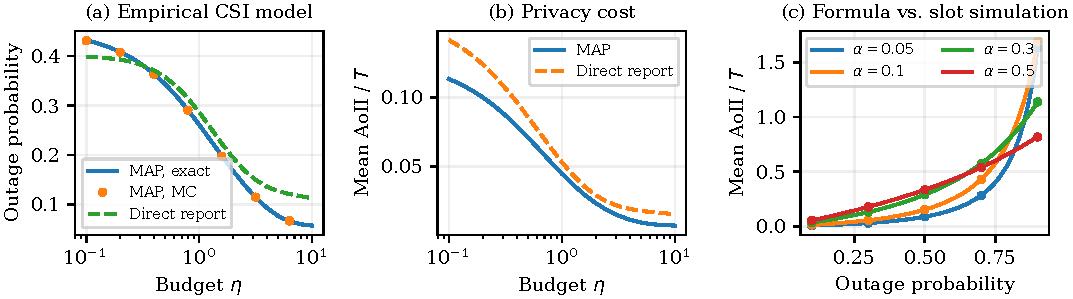
\includegraphics[width=\textwidth]{Figs/mechanism_theory.pdf}
\caption{Empirical-channel privacy cost and analytical validation. Solid MAP curves in (a) use analytical integration; markers and dashed direct-report curves use Monte Carlo (MC). In (c), lines are analytical and markers are direct task-state simulations with nominal pointwise 95\% batch-mean intervals for 36 controlled settings.}
\label{fig:mechanism}
\end{figure*}

\subsection{Fixed Privacy-Budget Selection}
Let $\mathcal E\subset(0,\infty)$ be a finite set of candidate budgets, fixed before testing. To select a common budget for a public distribution of hovering scenarios, specify weights $\omega_j\ge0$, $\sum_j\omega_j=1$, independently of the private test location, and define
\begin{equation}
 J(\epsilon)=\sum_{j=1}^{N_{\mathrm x}}\omega_j
           \overline\Delta_\epsilon^{\rm II}(\mathbf x_j).
 \label{eq:scenario-cost}
\end{equation}
Weights aggregate separate hovering sessions; the MAP prior governs inference within each session. AoII must be averaged after conditioning on location; applying~\eqref{eq:mean-aoii} to average outage generally differs.

Given a maximum single-report budget $\eta_{\max}$ at distance $r_0$, the primary problem is
\begin{equation}
 \begin{aligned}
 \mathrm{(P1)}\quad&\min_{\epsilon\in\mathcal E}&&J(\epsilon)\\
 &\mathrm{subject\ to}&&\epsilon r_0\le\eta_{\max}.
 \end{aligned}
 \label{eq:p1}
\end{equation}
Algorithm~\ref{alg:lapis} selects $\epsilon$ offline for the entire session. Repeated reports accumulate privacy loss across the session. For a finite session of $K$ reports with total budget $B_{\rm priv}$ under the repeated-location model, replace the constraint by $K\epsilon r_0\le B_{\rm priv}$. The selected budget remains fixed throughout the session.

An alternative design perspective prioritizes the strongest report protection compatible with an AoII requirement $D_{\max}$:
\begin{equation}
 \mathrm{(P2)}\quad
 \min_{\epsilon\in\mathcal E}\ \epsilon r_0
 \quad\mathrm{subject\ to}\quad J(\epsilon)\le D_{\max}.
 \label{eq:p2}
\end{equation}
Figure~\ref{fig:mechanism} evaluates the mechanism and AoII mapping. Problems (P1) and (P2) specify alternative requirements. If conditional outages decrease with $\epsilon$, the largest feasible budget solves (P1); no interior optimum is required. Otherwise, candidates are compared under identical link/source conditions, and the selected budget is independently confirmed.


